% TODO: Fix this subsection
\subsection{Bonds}
Source: \href{https://en.wikipedia.org/wiki/Chemical_bond}{Wiki: Chemical bond}

\subsubsection{Covalent bonding}
These type of bonds are made between non-metal elements.\\
Vdw Force is present

\begin{description}
    \item[non-polar] small electronegativity difference ($<$ 0.3)
    \item[polar] greater electronegativity difference, have dipole-dipole interaction\\
        Like $\text{H}_2\text{O}$\\
        Just means asymmetrical charge, but the total = 0
\end{description}

\subsubsection{Ionic bonding}
These type of bonds are made between non-metal and metal elements.
\\
Vdw Force is present\\
if H atoms on N/O/F/[Cl] the Hydrogen bond [H-Brücke] forces are present\\ 
The naming convention is cations than anions.\\

\begin{description}
    \item[] Salts
    \item[] Ions (Cations+,Anions-)
    \item[] Dissolved in water, they conduct electricity
    \item[] They are brittle [Spröd]
    \item[] NaCl \arrow sodium chloride
\end{description}
%
If we have N/S/P followed by O are nitrate/sulfate/phosphate which are anions.\\
Nitrate dissolve really easily in water.

\subsubsection{Metal bonding}
This bond is made between metal elements.

\begin{description}
    \item[] Atomic cores [Atomrümpfe]
    \item[] Electron gas \arrow give away valence electrons easily
    \item[] Generally electrically and heat conductive
\end{description}

\subsubsection{Geometry}
The shape of the molecule is determined by the central atom.
\\
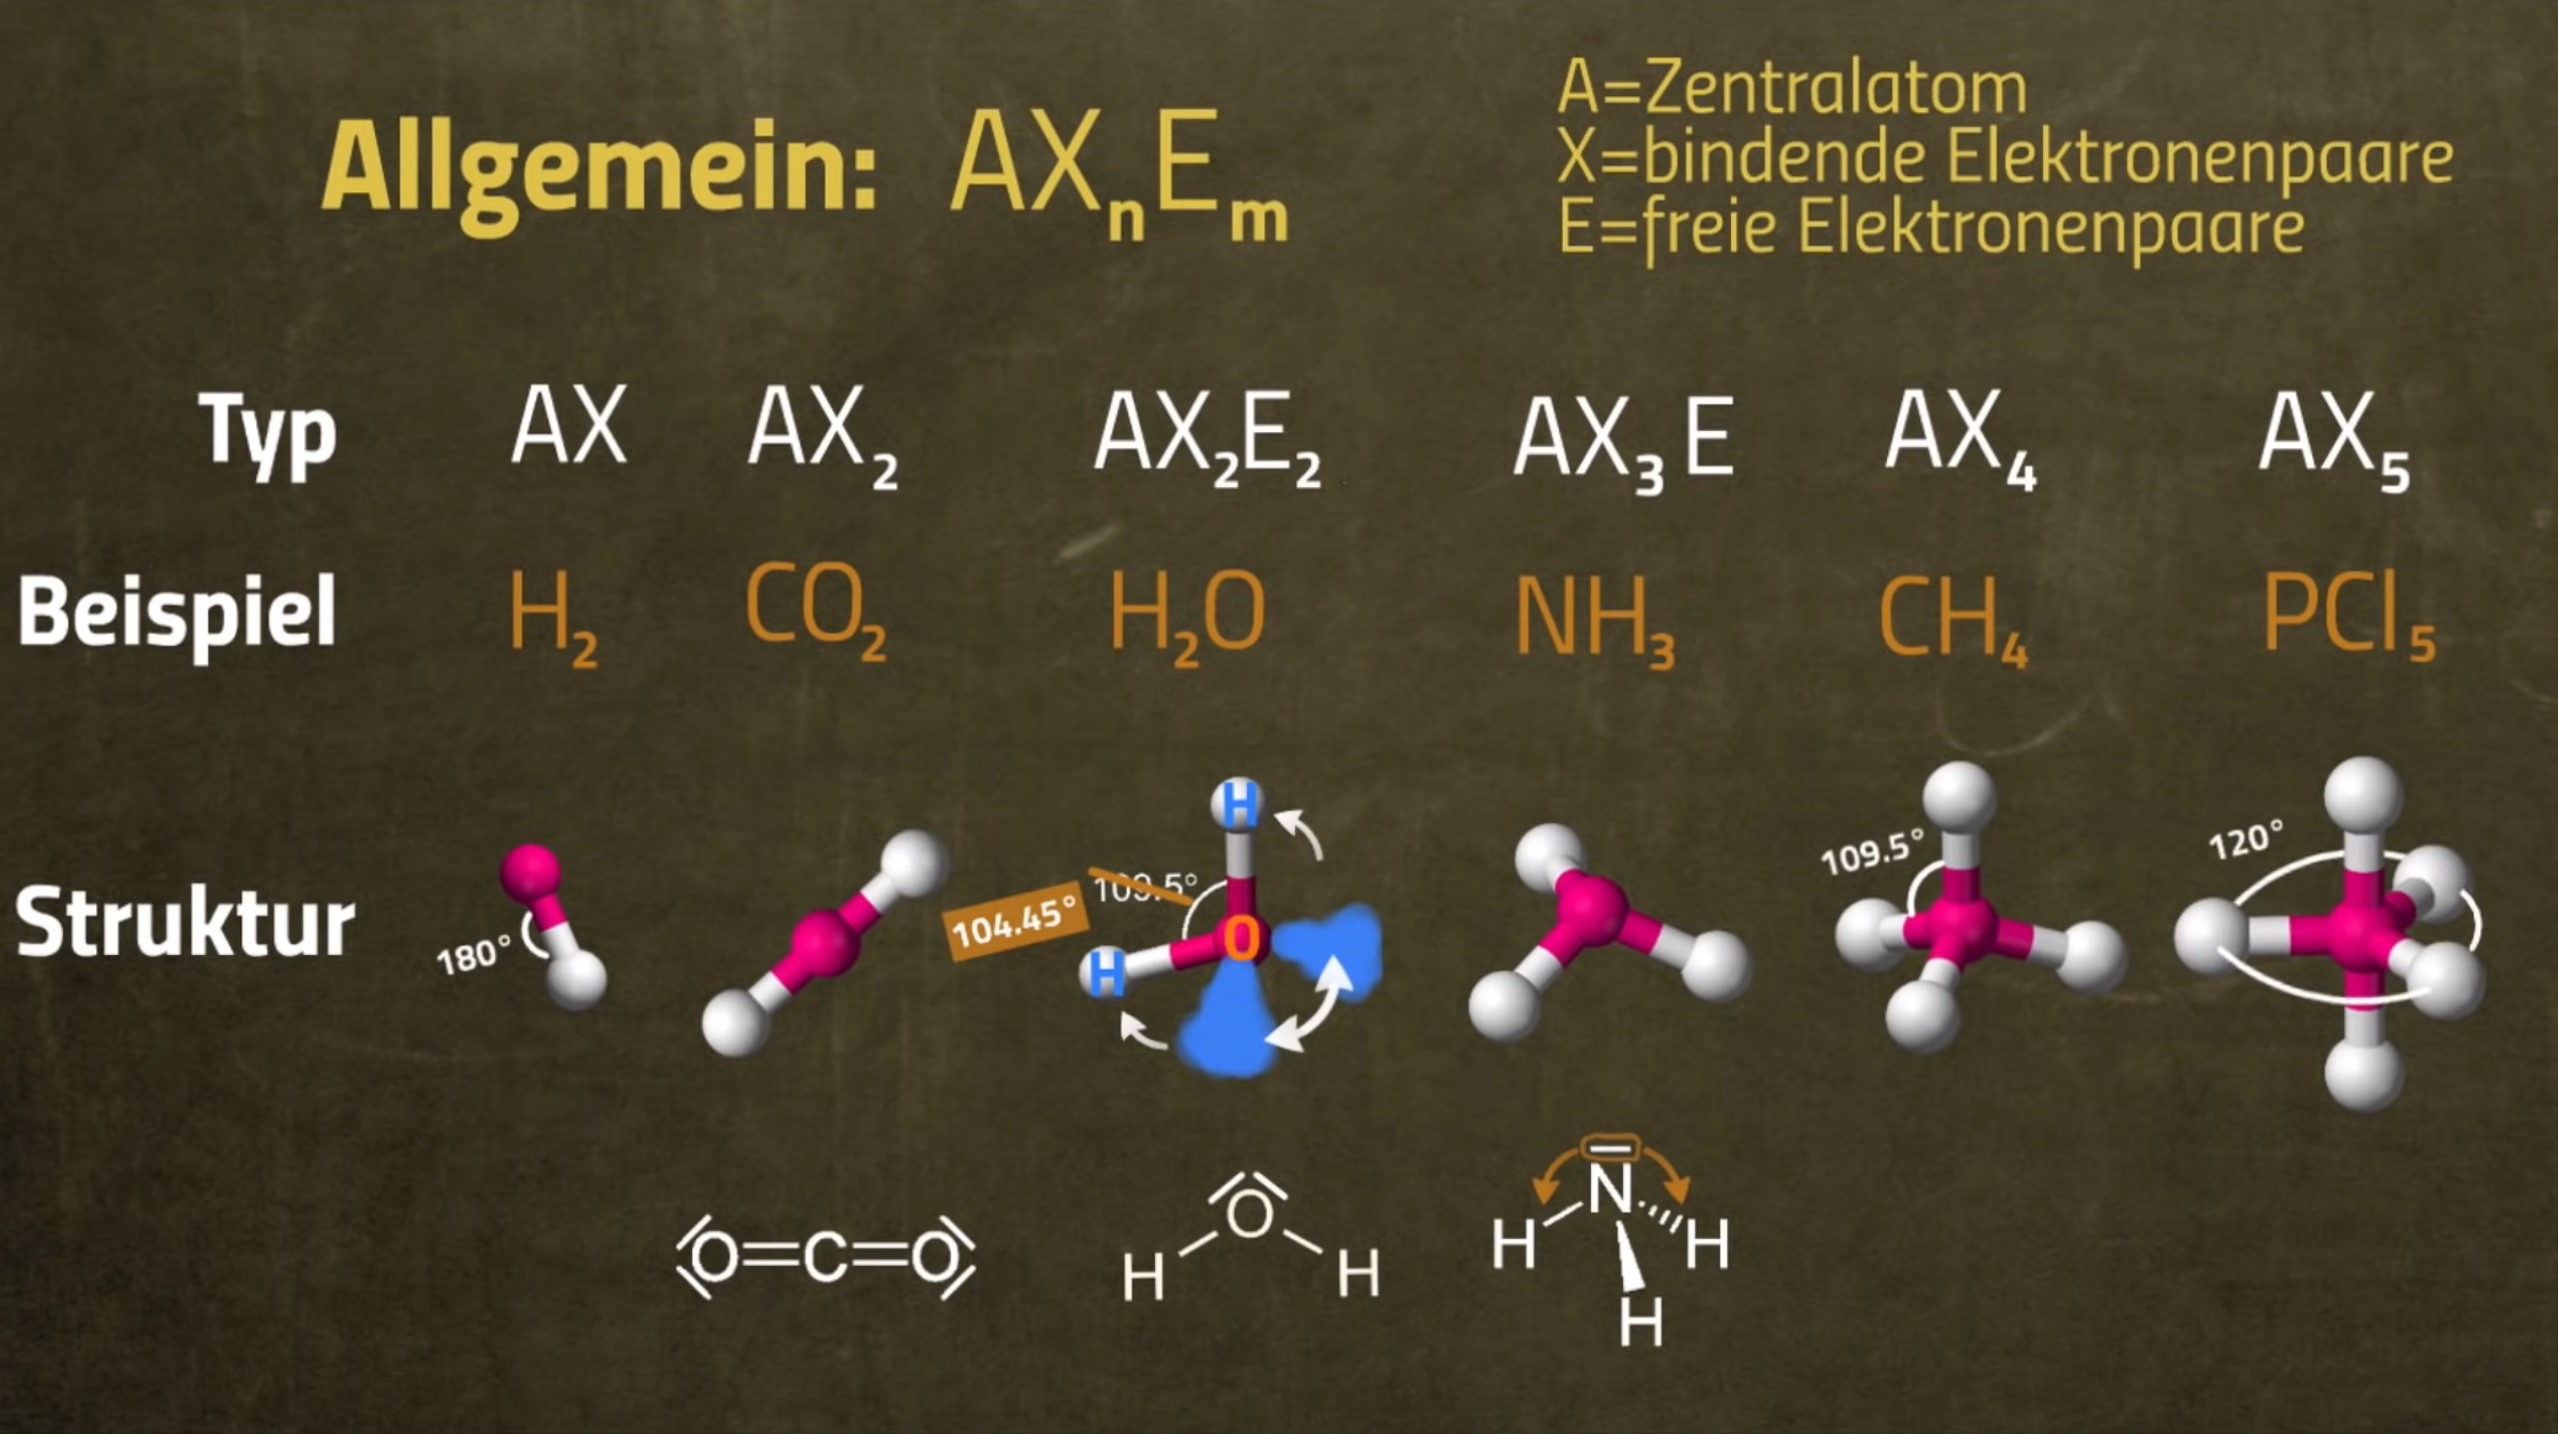
\includegraphics[width=30em]{./includes/chemistry/imgs/geometry.png}